% =========================================
\section{Modèle non-linéaire}
% =========================================
L'objectif de cette section est de généraliser le modèle EDP linéaire \eqref{modele_McKendrick_Lotka} en un modèle non-linéaire qui retranscrit plus fidèlement l'évolution de la population dans le temps.

\subsection{Modèle de Verhulst}
Comme pour la construction du modèle de McKendrick-Lotka \eqref{modele_McKendrick_Lotka}, on commence par étudier le modèle EDO introduit par Pierre François Verhulst qui généralise le modèle de Malthus. Le modèle de Verhulst fait l'hypothèse que le taux de natalité et le taux de mortalité sont des fonctions affines respectivement décroissante et croissante de la taille de la population. On note $P(t)$ le nombre d'individu d'une population à l'instant $t \in \bbR_+$. On conserve les notations $\beta$ et $\mu$ pour les taux de natalité et mortalité, mais on suppose cette fois que ce sont des fonctions de $P$. En s'inspirant du modèle de Malthus, on obtient l'équation 
\begin{equation*}
    P'(t) = \big(\beta(P)-\mu(P)\big)P(t)
\end{equation*}
Le fonction $P \mapsto \beta(P)-\mu(P)$ est le \textcolor{astral}{\textit{taux net de croissance}} de la population $P$. Verhulst propose qu’il diminue à mesure que la population augmente. L’observation du réel pousse également Verhulst à poser que pour de petits effectifs de population $P$, le taux net de croissance de cette population est strictement positif et potentiellement plutôt élevé (la population est initialement en croissance, car les conditions sont favorables avec des ressources abondantes). Tandis que pour de grands effectifs, le taux net de croissance tend à se réduire voire devenir nul (conditions défavorables à la croissance : vieillissement, concurrence accrue pour les ressources limitées).

Cette hypothèse revient à dire que pour $P$ tendant vers $0$ (population initiale), le taux net de croissance est positif. Ce taux étant une fonction affine décroissante de $P$ \textit{i.e.} $\beta(P)-\mu(P)=a-bP$, avec $a,b>0$. L'équation devient 
\begin{equation*}
    P'(t) = \big(a-bP(t)\big)P(t) = aP(t)-bP(t)^2
\end{equation*}
en posant $K=a/b >0$ la \textcolor{astral}{\textit{capacité d'accueil}}, que l'on suppose strictement positive dans notre contexte démographique, on obtient la forme \og logistique \fg{} de l'équation 
\begin{equation*}
    P'(t) = aP(t)\Big(1-\frac{P(t)}{K}\Big)
\end{equation*}
On remarque que $a=\beta-\mu>0$, où on reprend les notations introduites pour l'étude du modèle de Malthus. La solution du modèle de Verhulst est donnée par 
\begin{equation*}
    P(t) = K \frac{1}{1+\Big(\dfrac{K}{P(0)}-1\Big)\ex^{-at}}
\end{equation*}

\begin{remark}
    On observe que la population tend vers la capacité d'accueil $K$ quand $t$ tend vers $+\infty$ et que $P$ est croissante si la population initiale est inférieure à la population d'accueil et décroissante sinon.
\end{remark}

On peut chercher de potentiels points d'équilibre de ce modèle. Un point d'équilibre est une solution constante $P(t) \equiv P^*$. En remplaçant dans l'EDO, on obtient
\begin{eqnarray*}
    aP^*\Big(1-\frac{P^*}{K}\Big) = 0 &\iff& aP^* = 0 \ \text{ ou } \ 1-\frac{P^*}{K} = 0 \\
    &\iff& P^* = 0 \ \text{ ou } \ P^* = K
\end{eqnarray*}
on obtient deux solutions, $0$ et $K$. Ce sont les deux seuls points d'équilibre du modèle. \'Etudtions la stabilité de ces points d'équilibres. On introduit le champ de vecteur associé au modèle de Verhulst
\begin{equation*}
    F : \bbR \rightarrow \bbR, \ y \mapsto ay\Big(1-\frac{y}{K}\Big)
\end{equation*}
ce champ de vecteur est de classe $\scrC^1$ donc localement Lipschitzien. On introduit ensuite le flot associé au champ de vecteur $F$, qui est la solution du problème de Cauchy 
\begin{equation*}
    \left\{\begin{array}{l}
        P'(t) = F\big(P(t)\big) \\
        P(0)=x
    \end{array}\right.
\end{equation*}
donc le flot est défini pour tout $t \geq 0$ par 
\begin{equation*}
    \left\{\begin{array}{ll}
        \Phi(t,x) = K \bigg(1+\Big(\dfrac{K}{x}-1\Big)\ex^{-at}\bigg)^{-1} & \text{si } x \neq 0, \\
        \Phi(t,0) = 0 & \text{sinon.}
    \end{array}\right.
\end{equation*}

\begin{remark}
    Le champ de vecteur est complet.
\end{remark}

Il est clair que le point d'équilibre $0$ est stable, mais n'est pas localement asymptotiquement stable. En effet, la solution issue de la condition initiale $x=0$ reste identiquement nulle. Ainsi, le point d'équilibre $0$ n'est pas attractif. De même, le point d'équilibre $K$ n'est pas globalement attractif puisque la solution issue de la condition initiale $x=0$ reste identiquement nulle et ne converge donc pas vers $K$. Montrons maintenant que $K$ est localement asymptotiquement stable. Commençons d'abord par établir sa stabilité. Soit $\varepsilon>0$. Si $|x-K|<\varepsilon$, alors pour tout $t\geq0$
\begin{eqnarray*}
    |\Phi(t,x)-K| = K\bigg|\frac{1}{1+\Big(\dfrac{K}{x}-1\Big)\ex^{-at}}-1\bigg| \leq K\Big|\frac{x}{K}-1\Big| = |x-K| < \varepsilon
\end{eqnarray*}
donc $K$ est stable. Ensuite, en prenant $\varepsilon >0$ tel que $\varepsilon / K \geq 1$ par exemple $\varepsilon=K$. On a pour $|x-K| < \varepsilon$, $|x/K - 1| < \varepsilon/K$ donc 
\begin{equation*}
    \frac{K}{1+\dfrac{\varepsilon}{K}\ex^{-at}} \leq \Phi(t,x) \leq \frac{K}{1-\dfrac{\varepsilon}{K}\ex^{-at}}
\end{equation*}
en passant à la limite quand $t$ tend vers $0$, on obtient 
\begin{equation*}
    \lim_{t \to 0} \Phi(t,x) = K
\end{equation*}
Donc $K$ est localement asymptotiquement stable.

\begin{figure}[H]
\centering
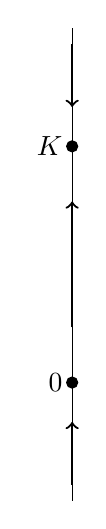
\begin{tikzpicture}[scale=1]

    % Axe
    \draw[-] (0,-3) -- (0,3);

    % Equilibres
    \filldraw (0,-1.5) circle (2pt);
    \filldraw (0,1.5) circle (2pt);

    % Labels
    \node[left] at (0,-1.5) {$0$};
    \node[left] at (0,1.5) {$K$};

    % Flèches
    \draw[->, thick] (0,-2.8) -- (0,-2.0);
    \draw[->, thick] (0,-0.8) -- (0,0.8);
    \draw[->, thick] (0,2.8) -- (0,2.0);

\end{tikzpicture}
\caption{Portraits de phase du modèle de Verhulst pour $x \neq 0$.}
\label{fig:portrait-verhulst}
\end{figure}

\subsection{Modèle de McKendrick-Lotka non-linéaire}
Dans cette section, nous allons introduire un modèle de McKendrick-Lotka non-linéaire en se basant sur le modèle EDO de Verhulst dont on a parlé précédemment. Donc en se basant sur la section précédente, on pourrait considérer l'équation 
\begin{equation*}
    \partial_tx(a,t)+\partial_ax(a,t) = -\mu(a)x(a,t)-\gamma(a)x(a,t)^2
\end{equation*}
où $\gamma \in L^\infty(0,a_{\max})$ et $\gamma > 0$, cette fonction peut représenter un terme de compétition inter-population (pour les ressources par exemple). Cependant, si on cherche à retrouver le modèle de Verhulst, on suppose $\beta$, $\mu$ et $\gamma$ constantes et on intègre par rapport à $a$ sur $[0,a_{\max}]$, on obtient 
\begin{eqnarray*}
    \int_0^{a_{\max}}\partial_tx(a,t)\d a+\int_0^{a_{\max}}\partial_ax(a,t)\d a = -\mu \int_0^{a_{\max}}x(a,t)\d a-\gamma \int_0^{a_{\max}}x(a,t)^2\d a
\end{eqnarray*}
on permutte intégrale et dérivée en temps et on obtient 
\begin{equation*}
    \frac{\d}{\d t} P(t) + x(a_{\max},t)-x(0,t) = -\mu P(t) - \gamma \int_0^{a_{\max}}x(a,t)^2\d a
\end{equation*}
on a $x(a_{\max},t)=0$ par hypothèse et avec la condition au bord, on obtient
\begin{equation*}
    P'(t) -\beta P(t) = -\mu P(t) -\gamma\int_0^{a_{\max}}x(a,t)^2\d a
\end{equation*}
finalement
\begin{equation*}
    P'(t) = (\beta-\mu)P(t) - \gamma \int_0^{a_{\max}}x(a,t)^2\d a
\end{equation*}
On ne retrouve pas le modèle de Verhulst avec cette équation, pour corriger cela on va plutôt considérer l'équation 
\begin{equation*}
    \partial_a x(a,t) + \partial_t x(a,t) = -\mu(a)x(a,t)-\gamma(a)\|x(\cdot,t)\|_{L^1}x(a,t)
\end{equation*}
où le terme $\|x(\cdot,t)\|_{L^1}$ permet au terme de compétition $\gamma$ d'agir sur l'entièreté de la population et pas seulement sur la densité de population d'âge $a$ à l'instant $t$. En reprenant les calculs précédents, on obtient 
\begin{equation*}
    P'(t) = (\beta-\mu)P(t) - \gamma P(t)^2
\end{equation*}
on retrouve alors le modèle de Verhulst. On considère alors le modèle non-linéaire de McKendrick-Lotka suivant
\begin{equation}\label{modele_McKendrick_Lotka_non_lineaire}
    \left\{\begin{array}{l}
        \partial_a x(a,t) + \partial_t x(a,t) = -\mu(a)x(a,t)-\gamma(a)\|x(\cdot,t)\|_{L^1}x(a,t) \\
        \\
        x(0,t) = B(t) = \displaystyle{\int_0^{a_{\max}}} \beta (a)x(a,t)\d a \\
        \\
        x(a,0) = x_0(a)
    \end{array}\right.
\end{equation}

\subsection{Existence et unicité}
On se demande à présent si on a existence et/ou unicité de solutions au modèle \eqref{modele_McKendrick_Lotka_non_lineaire}. On va chercher à mettre le modèle \eqref{modele_McKendrick_Lotka_non_lineaire} sous la forme \eqref{pbmCauchy_semilineaire} afin d'utiliser le théorème \ref{CauchyLipschitz_explosiontempsfini}. Comme dans la section précédente, on considère $x: \bbR_+ \rightarrow L^1(0,a_{\max})$ et l'opérateur $A$. Et donc on a 
\begin{equation*}
    \left\{\begin{array}{l}
        \dfrac{\d}{\d t}x(t) = Ax(t) -\gamma\|x(t)\|_{L^1}x(t) \\
        \\
        x(0) = x_0
    \end{array}\right.
\end{equation*}
On pose alors 
\begin{eqnarray*}
    f : \bbR_+ \times L^1(0,a_{\max}) \rightarrow L^1(0,a_{\max}), \ (t,u) \mapsto - \gamma \|u\|_{L^1}u
\end{eqnarray*}
de sorte à obtenir le problème 
\begin{equation}\label{pbmCauchy_McKendrick_Lotka_non_lineaire}
    \left\{\begin{array}{l}
        \dfrac{\d}{\d t}x(t) = Ax(t) + f\big(t,x(t)\big) \\
        \\
        x(0) = x_0
    \end{array}\right.
\end{equation}
\begin{remark}
    Ici, on définit $f$ sur $\bbR_+ \times L^1(0,a_{\max})$ pour coller avec les hypothèses du théorème \ref{CauchyLipschitz_explosiontempsfini}, mais une fois ce théorème appliquer et le résultat d'existence et unicité obtenu, on notera plu simplement $f : L^1(0,a_{\max}) \rightarrow L^1(0,a_{\max}), \ u \mapsto -\gamma \|u\|_{L^1}u$.
\end{remark}

\begin{theorem}
    Le problème \eqref{pbmCauchy_McKendrick_Lotka_non_lineaire} admet une unique solution mild dans $L^1(0,a_{\max})$.
\end{theorem}

\begin{proof}
    On sait déjà que $A$ est le générateur du $\scrC^0$ semi-groupe $\big\{T(t)\big\}_{t \geq 0}$. La fonction $f$ est clairement continue en $t$, il nous reste à vérifier qu'elle est localement Lipschitz en $u$, uniformément en $t$ sur les compacts. Soient $t_0 \in \bbR_+$ et $R>0$. Soient $u,v \in \overline{B_{L^1}(0,R)}$ et $t \in [0,t_0]$. On a 
    \begin{eqnarray*}
        \|f(t,u)-f(t,v)\|_{L^1} &=& \big\|\gamma \big(\|u\|_{L^1}u-\|v\|_{L^1}v\big)\big\|_{L^1} \\
        &\leq& \|\gamma\|_{L^\infty}\big\|\|u\|_{L^1}u-\|v\|_{L^1}v\big\|_{L^1} \\
        &=& \|\gamma\|_{L^\infty}\big\|\|u\|_{L^1}(u-v)+\big(\|u\|_{L^1}-\|v\|_{L^1}\big)v\big\|_{L^1} \\
        &\leq& \|\gamma\|_{L^\infty}\big(\|u\|_{L^1}\|u-v\|_{L^1}+\big|\|u\|_{L^1}-\|v\|_{L^1}\big|\|v\|_{L^1}\big) \\
        &\leq& \|\gamma\|_{L^\infty}\big(\|u\|_{L^1}+\|v\|_{L^1}\big)\|u-v\|_{L^1} \\
        &\leq& 2\|\gamma\|_{L^\infty}R\|u-v\|_{L^1}
    \end{eqnarray*}
    donc $f$ est bien localement Lipschitz en $u$, uniformément en $t$ sur les compacts. On peut donc appliquer le théorème \ref{CauchyLipschitz_explosiontempsfini}. Ainsi, pour tout $x_0 \in L^1(0,a_{\max})$, il existe $t_{\max} >0$ tel que le problème \eqref{pbmCauchy_McKendrick_Lotka_non_lineaire} admet une unique solution mild $x$ sur $[0,t_{\max}[$ donnée par 
    \begin{eqnarray}\label{sol_mild_non_lineaire}
        x(t) &=& T(t)x_0 + \int_0^t T(t-s)f\big(s,x(s)\big)\d s \nonumber \\
        &=& T(t)x_0 - \int_0^t \|x(s)\|_{L^1}T(t-s)\big(\gamma x(s)\big)\d s
    \end{eqnarray}
\end{proof}

\begin{corollaire}
    La solution mild \eqref{sol_mild_non_lineaire} du problème \eqref{pbmCauchy_McKendrick_Lotka_non_lineaire} est globale.
\end{corollaire}

\begin{proof}
    Supposons par l'absurde que $t_{\max} <+\infty$ alors par le théorème \ref{CauchyLipschitz_explosiontempsfini}, on a 
    \begin{equation*}
        \lim_{t \to t_{\max}}\|x(t)\|_{L^1}=+\infty
    \end{equation*}
    Comme le semi-groupe $\big\{T(t)\big\}_{t \geq 0}$ est positif, on a 
    \begin{equation*}
        x(t) \leq T(t)x_0
    \end{equation*}
    donc 
    \begin{eqnarray*}
        \|x(t)\|_{L^1} \leq \|T(t)x_0\|_{L^1} &\Longrightarrow& \|x(t)\|_{L^1} \leq \ex^{\|\beta\|_{L^\infty}t}\|x_0\|_{L^1}
    \end{eqnarray*}
    ainsi, en passant à la limite quand $t$ tend vers $t_{\max}$ on obtient 
    \begin{equation*}
        +\infty = \lim_{t \to t_{\max}} \|x(t)\|_{L^1} \leq \ex^{t_{\max}\|\beta\|_{L^\infty}}\|x_0\|_{L^1}<+\infty
    \end{equation*}
    ce qui est absurde, donc $t_{\max}=+\infty$. La solution mild donnée par \eqref{sol_mild_non_lineaire} est donc globale.
\end{proof}

\begin{proposition}
    La solution mild \eqref{sol_mild_non_lineaire} est positive.
\end{proposition}

\begin{proof}
    Soit $c \in \bbR$. On écrit 
    \begin{equation*}
        A+f = A-cI + cI +f
    \end{equation*}
    L'objectif est de déterminer un $c$ tel que $cI+f$ soit, localement, un opérateur positif et $A-cI$ génère toujours un $\scrC^0$ semi-groupe positif. Soit $R>0$. On cherche donc $c$ tel que 
    \begin{equation*}
        \big(cI+f\big)\big(B_{L^1}(0,R)\cap L^1_+(0,a_{\max})\big) \subset L^1_+(0,a_{\max})
    \end{equation*}
    Soit $x \in B_{L^1}(0,R)\cap L^1_+(0,a_{\max})$. On a 
    \begin{eqnarray*}
        (cI+f)(x) = cx+f(x) = cx-\gamma\|x\|_{L^1}x
    \end{eqnarray*}
    Pour que $(cI+f)(x) \geq 0$, il suffit de prendre $c:=\|\gamma\|_{L^\infty}R$. On sait que $A$ génère un $\scrC^0$ semi-groupe et comme $cI$ est un opérateur uniformément borné, il génère le semi-groupe uniformément continu $\{\ex^{ct}\}_{t\geq 0}$. Donc on a 
    \begin{eqnarray*}
        A-cI &=&\lim_{t \to 0}\frac{T(t)-I}{t} - \lim_{t \to 0} \frac{\ex^{ct}-I}{t} \\
        &=& \lim_{t \to 0} \frac{T(t)-I-\ex^{ct}+I}{t} \\
        &=& \lim_{t \to 0} \frac{T(t)-\ex^{ct}}{t} \\
        &=& \lim_{t \to 0} \frac{1}{\ex^{-ct}}\frac{\ex^{-ct}T(t)-I}{t} \\
        &=& \lim_{t \to 0} \frac{\ex^{-ct}T(t)-I}{t}
    \end{eqnarray*}
    donc $A-cI$ génère le $\scrC^0$ semi-groupe $\big\{\ex^{-ct}T(t)\big\}_{t \geq 0}$, ce semi-groupe est clairement positif. Le problème \eqref{pbmCauchy_McKendrick_Lotka_non_lineaire} est équivalent au problème suivant 
    \begin{equation*}
        \left\{\begin{array}{l}
        \dfrac{\d}{\d t}u(t) = (A-cI)u(t) + (cI+f)u(t) \\
        \\
        u(0) = x_0
    \end{array}\right.
    \end{equation*}
    Ce problème admet une unique solution mild par le théorème \ref{CauchyLipschitz_explosiontempsfini} et cette solution est donnée par 
    \begin{equation*}
        u(t) = \ex^{-ct}T(t)x_0 + \int_0^t \ex^{-c(t-s)}T(t-s)(cI+f)u(s)\d s
    \end{equation*}
    On pose à présent 
    \begin{eqnarray*}
        F : \scrC^0\big(\bbR_+,L^1(0,a_{\max})\big) &\rightarrow& \scrC^0\big(\bbR_+,L^1(0,a_{\max})\big) \\
        u &\mapsto& (Fu)(t)=\ex^{-ct}T(t)x_0 + \int_0^t \ex^{-c(t-s)}T(t-s)(cI+f)u(s)\d s
    \end{eqnarray*}
    Et $F$ préserve le cône positif $L^1_+(0,a_{\max})$, en effet si $u \geq 0$, alors on a montré que $(cI+f)u \geq 0$ et comme $T(t)$ est positif $(Fu)(t) \geq 0$. La solution étant construite par itérée de Picard, si on choisit $x_0 \geq 0$, alors toutes les itérations restent positives et donc $u(t) \geq 0$. Finalement, comme $u(t)$ est positive, $x(t)$ l'est aussi.
\end{proof}

\subsection{Points d'équilibre et stabilité}
L'objectif de cette section est de déterminer l'existence ou non de point d'équilibre pour $A+f$, d'étudier la nature de ces potentiels points d'équilibres et d'interpréter ces résultats.
\paragraph{Points d'équilibre.} Déterminer les points d'équilibres revient à chercher une solution $x_0 \in D(A)$ de notre EDP qui ne dépend pas du temps. En injectant $x_0$ dans l'EDP de \eqref{pbmCauchy_McKendrick_Lotka_non_lineaire}, on obtient 
\begin{equation*}
    Ax_0+f(x_0) = 0
\end{equation*}
donc 
\begin{eqnarray*}
    -x_0'-\mu x_0 -\gamma \|x_0\|_{L^1}x_0 = 0 &\iff& x_0' = -(\mu + \gamma \|x_0\|_{L^1})x_0
\end{eqnarray*}
La solution de cette EDO est donnée par 
\begin{equation*}
    x_0(a) = x_0(0)\Pi(a)\exp\bigg(-\|x_0\|_{L^1}\int_0^a\gamma(\sigma)\d \sigma\bigg)
\end{equation*}
Comme $x_0 \in D(A)$, en injectant l'expression de $x_0$ dans la condition au bord, on a
\begin{eqnarray*}
    x_0(0) = x_0(0)\int_0^{a_{\max}}\beta(a)\Pi(a)\exp\bigg(-\|x_0\|_{L^1}\int_0^a\gamma(\sigma)\d \sigma\bigg)\d a 
\end{eqnarray*}
donc 
\begin{equation*}
    x_0(0)\bigg(1-\int_0^{a_{\max}}K(a)\exp\bigg(-\|x_0\|_{L^1}\int_0^a \gamma(\sigma)\d \sigma\bigg)\d a\bigg) = 0
\end{equation*}
On a alors deux cas
\begin{enumerate}
    \item $x_0(0)=0$, alors $x_0\equiv 0$ et donc le seul point d'équilibre est $0$.
    \item sinon, on a 
    \begin{equation}\label{eq_pts_equilibres}
        \int_0^{a_{\max}}K(a)\exp\bigg(-\|x_0\|_{L^1}\int_0^a\gamma(\sigma)\d \sigma\bigg)\d a = 1
    \end{equation}
    \begin{remark}
        On peut alors déterminer complétement $x_0$, en effet l'équation précédente nous permet de déterminer $\|x_0\|_{L^1}$. Puis, on peut déterminer $x_0(0)$, en effet 
        \begin{eqnarray*}
            \|x_0\|_{L^1} &=& \int_0^{a_{\max}} x_0(a)\d a \\
            &=& x_0(0) \int_0^{a_{\max}} \Pi(a)\exp\bigg(-\|x_0\|_{L^1}\int_0^a\gamma(\sigma)\d\sigma\bigg)\d a
        \end{eqnarray*}
        donc 
        \begin{equation}\label{eq_deter_x0}
            x_0(0) = \frac{\|x_0\|_{L^1}}{\displaystyle{\int_0^{a_{\max}}\Pi(a)\exp\bigg(-\|x_0\|_{L^1}\displaystyle{\int_0^a}\gamma(\sigma)\d\sigma\bigg)\d a}}
        \end{equation}
    \end{remark}
    On peut à présent revenir à l'étude des points d'équilibres. Pour déterminer ceux-ci, on doit étudier la fonction 
    \begin{equation*}
        g : \bbR_+ \rightarrow \bbR, \ y \mapsto \int_0^{a_{\max}}K(a)\exp\bigg(-y\int_0^a\gamma(\sigma)\d \sigma\bigg)\d a
    \end{equation*}
    Cette fonction est clairement positive, continue et dérivable de dérivée 
    \begin{equation*}
        g'(y) = -\int_0^{a_{\max}}K(a)\gamma(a)\exp\bigg(-y\int_0^a\gamma(\sigma)\d \sigma\bigg)\d a < 0
    \end{equation*}
    Comme $\gamma > 0$, $g$ est strictement décroissante. De plus, on a 
    \begin{eqnarray*}
        g(0) = \int_0^{a_{\max}}K(a)\d a = R \ \ \ &\text{ et }& \ \ \ \lim_{y \to +\infty}g(y) = 0
    \end{eqnarray*}
    Si $R\leq1$, alors il n'y a pas de point d'équilibre non-trivial car pas de solution à l'équation \eqref{eq_pts_equilibres}. Si $R > 1$ alors $g$ étant continue, strictement décroissante et tendant vers $0$ à l'infini, on a par le TVI l'existence d'une unique solution $y^*\geq 0$ à l'équation \eqref{eq_pts_equilibres} et donc d'un unique point d'équilibre vérifiant
    \begin{equation*}
        \|x_0\|_{L^1}=y^*
    \end{equation*}
    et la solution est 
    \begin{equation*}
        x_0(a)=x_0(0)\Pi(a)\exp\bigg(-y^*\int_0^a\gamma(\sigma)\d \sigma\bigg)
    \end{equation*}
    avec $x_0(0)$ déterminé par \eqref{eq_deter_x0}.
\end{enumerate}

\paragraph{Stabilité.} On va à présent étudier la stabilité de ces points d'équilibre l'objectif étant d'utiliser la proposition \ref{prop_stab_pts_equilibre}. Soit $x_0$ un point d'équilibre. Tout d'abord, il nous faut calculer la dérivée en $x_0$ de $f$. Soit $x \in L^1_+(0,a_{\max})$, on fait cette hypothèse supplémentaire pour simplifier le calcul de la dérivée car dans notre contexte de dynamique des populations, la population initiale sera toujours positive. On a donc
\begin{eqnarray*}
    f(x+x_0)-f(x_0) &=& -\gamma \|x+x_0\|_{L^1}(x+x_0)+\gamma \|x_0\|_{L^1}x_0 \\
    &=& -\gamma \big(\|x+x_0\|_{L^1}-\|x_0\|_{L^1}\big)x_0 -\gamma \|x+x_0\|_{L^1}x \\
    &=& \underbrace{-\gamma x_0\int_0^{a_{\max}}x(a)\d a - \gamma \|x_0\|_{L^1}x}_{=:f'(x_0)x} \underbrace{- \gamma \|x\|_{L^1}x}_{=o(x)}
\end{eqnarray*}
d'où l'expression de la dérivée de $f$. On considère à présent l'opérateur 
\begin{equation*}
    \hat{A} := A + f'(x_0)
\end{equation*}

\begin{proposition}
    L'opérateur $\hat{A}$ est le générateur d'un $\scrC^0$ semi-groupe.
\end{proposition}

\begin{proof}
    On va appliquer la théorème \ref{thm_perturbation_operateur_borne}. Pour ça on vérifie que $f'(x_0)$ est continue sur $L^1_+(0,a_{\max})$, soit $x \in L^1_+(0,a_{\max})$ on a 
    \begin{eqnarray*}
        \|f'(x_0)x\|_{L^1} \leq 2\|\gamma\|_{L^\infty}\|x_0\|_{L^1}\|x\|_{L^1} \Longrightarrow \vertiii{f'(x_0)}_{L^1} \leq 2\|\gamma\|_{L^\infty}\|x_0\|_{L^1}
    \end{eqnarray*}
    en prenant $x=\dfrac{x_0}{\|x_0\|_{L^1}}$, on a 
    \begin{equation*}
        \|f'(x_0)x\|_{L^1} = 2\|\gamma\|_{L^\infty}\|x_0\|_{L^1}
    \end{equation*}
    donc 
    \begin{equation*}
        \vertiii{f'(x_0)}_{L^1} = 2\|\gamma\|_{L^\infty}\|x_0\|_{L^1}
    \end{equation*}
    donc par le théorème \ref{thm_perturbation_operateur_borne}, l'opérateur $\hat{A}$ est le générateur infinitésimal d'un $\scrC^0$ semi-groupe $\big\{S(t)\big\}_{t \geq 0}$ tel que 
    \begin{equation*}
        \forall t \geq 0, \ \vertiii{S(t)}_{L^1} \leq \ex^{\big(\|\beta\|_{L^\infty}+ 2\|\gamma\|_{L^\infty}\|x_0\|_{L^1}\big)t}
    \end{equation*}
\end{proof}

On s'intéresse à la relation entre le semi-groupe $\big\{T(t)\big\}_{t \geq 0}$ et le semi-groupe $\big\{S(t)\big\}_{t \geq 0}$. On considère l'opérateur $H(s):=T(t-s)S(s)$. Pour $x \in D(A)$, $s \mapsto H(s)x$ est différentiable et $H'(s)x = T(t-s)f'(x_0)S(s)x$. En intégrant cette équation par rapport à $s$ entre $0$ et $t$ on obtient 
\begin{eqnarray*}
    S(t)x-T(t)x = \int_0^tT(t-s)f'(x_0)S(s)x\d s &\iff& S(t)x=T(t)x+\int_0^tT(t-s)f'(x_0)S(s)x\d s
\end{eqnarray*}
Comme les opérateurs de chaque côtés de l'égalité sont bornés, cette égalité est vraie pour tout $x \in L^1(0,a_{\max})$ et $S(t)$ est une solution de cette équation intégrale.

\begin{proposition}\label{prop_res_compact_A_chapeau}
    La résolvante $R(\lambda : \hat{A})$ est compacte pour $\lambda > 2\|\gamma\|_{L^\infty}\|x_0\|_{L^1}+\alpha^*$ où $\lambda \in \rho(A)$.
\end{proposition}

\begin{proof}
    Commençons d'abord par écrire $R(\lambda : \hat{A})$ autrement. On a 
    \begin{eqnarray*}
        \lambda - \hat{A} = \lambda - A - f'(x_0) = \big(I-f'(x_0)R(\lambda : A)\big)(\lambda - A)
    \end{eqnarray*}
    donc $\lambda - \hat{A}$ est inversible si et seulement si $I-f'(x_0)R(\lambda : A)$ est inversible. Or, $\lambda >2\|\gamma\|_{L^\infty}\|x_0\|_{L^1}+\alpha^*$, donc
    \begin{eqnarray*}
        \vertiii{f'(x_0)R(\lambda : A)}_{L^1} \leq \vertiii{f'(x_0)}_{L^1}\vertiii{R(\lambda : A)}_{L^1}
        \leq \frac{2\|\gamma\|_{L^\infty}\|x_0\|_{L^1}}{\lambda - \alpha^*} < 1
    \end{eqnarray*}
    donc 
    \begin{equation*}
        \big(I-f'(x_0)R(\lambda : A)\big)^{-1} = \sum_{k=0}^{+\infty}\big(f'(x_0)R(\lambda : A)\big)^k
    \end{equation*}
    ce qui donne finalement
    \begin{equation*}
        R(\lambda : \hat{A}) = \sum_{k=0}^{+\infty}R(\lambda:A)\big(f'(x_0)R(\lambda:A)\big)^k
    \end{equation*}
    Montrons à l'aide de cette identité de $R(\lambda : \hat{A})$ est compacte. Soit $k \in \bbN$, le terme 
    \begin{equation*}
        R(\lambda : A)\big(f'(x_0)R(\lambda:A)\big)^k
    \end{equation*}
    est compact, comme produit d'un borné et d'un compact. Donc pour tout $k \in \bbN$, $R(\lambda : A)\big(f'(x_0)R(\lambda:A)\big)^k \in \scrK\big(L^1(0,a_{\max})\big)$. Et on sait que $\scrK\big(L^1(0,a_{\max})\big)$ est un sous-espace vectoriel fermé de $\scrL\big(L^1(0,a_{\max})\big)$ donc la série 
    \begin{equation*}
        \sum_{k=0}^{+\infty}R(\lambda:A)\big(f'(x_0)R(\lambda:A)\big)^k
    \end{equation*}
    converge dans $\scrK\big(L^1(0,a_{\max})\big)$, par conséquent $R(\lambda : \hat{A})$ est un opérateur compact.
\end{proof}

\begin{proposition}
    Le semi-groupe $\big\{S(t)\big\}_{t \geq 0}$ est éventuellement compact pour $t > a_{\max}$.
\end{proposition}

\begin{proof}
    On sait déjà par la proposition précédente que $R(\lambda : \hat{A})$ est compacte. Il nous suffit donc de montrer que $t \mapsto S(t)$ est continue pour la norme d'opérateur pour tout $t > a_{\max}$, le résultat sera alors donné par le théorème \ref{thm_SG_compact_res}. Soient $x \in L^1(0,a_{\max}) \setminus \{0\}$ et $t >a_{\max}$. On pose $M:=2\|\gamma\|_{L^\infty}\|x_0\|_{L^1}$ pour plus de lisibilité.
    \begin{eqnarray*}
        \|S(t+h)x-S(t)x\|_{L^1} &\leq& \|T(t+h)x-T(t)x\|_{L^1}+\bigg\|\int_0^{t+h}T(t+h-s)f'(x_0)S(s)x\d s \\
        &-& \int_0^t T(t-s)f'(x_0)S(s)x\d s\bigg\|_{L^1} \\
        &\leq& \vertiii{T(t+h)-T(t)}_{L^1}\|x\|_{L^1} \\
        &+& \bigg\| \int_0^t \big(T(t+h-s)-T(t-s)\big)f'(x_0)S(s)x\d s \\
        &+& \int_t^{t+h}T(t+h-s)f'(x_0)S(s)x\d s \bigg\|_{L^1} \\
        &\leq& \vertiii{T(t+h)-T(t)}_{L^1}\|x\|_{L^1}\\
        &+& M\|x\|_{L^1}\int_t^{t+h}\ex^{\|\beta\|_{L^\infty}(t+h-s)}\ex^{\big(\|\beta\|_{L^\infty}+M\big)s}\d s \\
        &+&M\|x\|_{L^1}\int_0^t\vertiii{T(t+h-s)-T(t-s)}_{L^1}\ex^{\big(\|\beta\|_{L^\infty}+M\big)s}\d s \\
        &=& \vertiii{T(t+h)-T(t)}_{L^1}\|x\|_{L^1} + \|x\|_{L^1}\ex^{\|\beta\|_{L^\infty}(t+h)}\big(\ex^{M(t+h)}-\ex^{Mt}\big) \\
        &+&M\|x\|_{L^1}\int_0^t\vertiii{T(t+h-s)-T(t-s)}_{L^1}\ex^{\big(\|\beta\|_{L^\infty}+M\big)s}\d s
    \end{eqnarray*}
    d'où 
    \begin{eqnarray*}
        \vertiii{S(t+h)-S(t)}_{L^1} &\leq& \vertiii{T(t+h)-T(t)}_{L^1} + \ex^{\|\beta\|_{L^\infty}(t+h)}\big(\ex^{M(t+h)}-\ex^{Mt}\big) \\
        &+& M \int_0^t\vertiii{T(t+h-s)-T(t-s)}_{L^1}\ex^{\big(\|\beta\|_{L^\infty}+M\big)s}\d s
    \end{eqnarray*}
    En passant à la limite quand $h$ tend vers $0$, on obtient par la proposition \ref{SG_T_compact} et par convergence dominée 
    \begin{equation*}
        \lim_{h \to 0} \vertiii{S(t+h)-S(t)}_{L^1} = 0
    \end{equation*}
    d'où la continuité du semi-groupe $\big\{S(t)\big\}_{t \geq 0}$ pour la norme d'opérateur pour tout $t >a_{\max}$ et donc l'éventuelle compacité.
\end{proof}

\begin{corollaire}
    On a $\omega_{\text{ess}}(\hat{A}) = -\infty$ et $\sigma_{\text{ess}}(\hat{A}) = \emptyset$.
\end{corollaire}

\begin{proof}
    Comme le semi-groupe $\big\{S(t)\big\}_{t \geq 0}$ est éventuellement compact, on a $\omega_{\text{ess}}(\hat{A}) = -\infty$. De plus, on a par le point $1$ de la proposition \ref{prop_lien_type_borne_spectrale} que 
    \begin{equation*}
        \sup\{\Re(\lambda) \in \bbR \ | \ \lambda \in \sigma_{\text{ess}}(\hat{A})\} \leq -\infty
    \end{equation*}
    donc $\sigma_{\text{ess}}(\hat{A})=\emptyset$.
\end{proof}

On pose 
\begin{equation*}
    \Phi(a) := \exp\bigg(-\|x_0\|_{L^1}\int_0^a\gamma(\sigma)\d \sigma\bigg)
\end{equation*}
cette fonction est une mortalité supplémentaire due à la compétition intra-population.

\begin{theorem}\label{thm_spectre_A_chapeau}
    On a 
    \begin{equation*}
        \sigma(\hat{A}) = \mathrm{VP}(\hat{A}) = \big\{\lambda \in \bbC \ | \ \widehat{K\Phi}(\lambda)=1\big\}
    \end{equation*}
    L'équation $\widehat{K\Phi}(\lambda)=1$ admet une unique solution réelle $\lambda^*$ qui vérifie $\lambda^*=s(\hat{A})$, c'est-à-dire que c'est la plus grande valeur propre de $\hat{A}$. De plus, on a $s(\hat{A}) \leq s(A)$.
\end{theorem}

\begin{proof}
    Commençons par identifier $\sigma(\hat{A})$. Soit $\lambda \in \rho(\hat{A})$. On cherche à résoudre l'équation d'inconnue $u$
    \begin{eqnarray*}
        R(\lambda:\hat{A})g = u &\iff& (\lambda I-\hat{A})u=g \\
        &\iff& \lambda u +\mu u +u' + \gamma x_0 \int_0^{a_{\max}}u(\sigma)\d \sigma + \gamma \|x_0\|_{L^1}u=g \\
        &\iff& u' = -\big(\lambda + \mu + \gamma \|x_0\|_{L^1}\big)-\gamma x_0 \int_0^{a_{\max}}u(\sigma)\d \sigma + g \\
        &\iff& u(a) = \ex^{-\lambda a}\Pi(a)\Phi(a)\bigg(u(0)+\int_0^a \frac{g(s)-\gamma(s)x_0(s)\displaystyle{\int_0^{a_{\max}} u(\sigma)\d \sigma}}{\Phi(s)}\d s\bigg)
    \end{eqnarray*}
    La condition au bord nous donne 
    \begin{eqnarray*}
        u(0) = \int_0^{a_{\max}}\beta(a)u(a)\d a &\iff& u(0)=\int_0^{a_{\max}}\ex^{-\lambda a}K(a)\Phi(a)\d a \\
        &+& \int_0^{a_{\max}}\ex^{-\lambda}K(a)\Phi(a)\int_0^a \frac{g(s)-\gamma(s)x_0(s)\displaystyle{\int_0^{a_{\max}} u(\sigma)\d \sigma}}{\Phi(s)}\d s \\
        &\iff& u(0)\big(1-\widehat{K\Phi}(\lambda)\big) = \int_0^{a_{\max}}\ex^{-\lambda}K(a)\Phi(a) \\
        &\times& \int_0^a \frac{g(s)-\gamma(s)x_0(s)\displaystyle{\int_0^{a_{\max}} u(\sigma)\d \sigma}}{\Phi(s)}\d s
    \end{eqnarray*}
    Cette équation admet une unique solution si et seulement si $\widehat{K\Phi}(\lambda) \neq 1$. On peut ensuite déterminer $\|u\|_{L^1}$, 
    \begin{eqnarray*}
        \|u\|_{L^1} = \int_0^{a_{\max}}u(a)\d a &\iff& \|u\|_{L^1} = \int_0^{a_{\max}}\ex^{-\lambda a}\Pi(a)\Phi(a)\bigg(u(0)\\
        &+& \int_0^a \frac{g(s)-\gamma(s)x_0(s)\|u\|_{L^1}}{\Phi(s)}\d s\bigg) \d a \\
        &\iff& \|u\|_{L^1}\bigg(1+\int_0^{a_{\max}}\int_0^a \frac{\gamma(s)x_0(s)}{\Phi(s)}\d s\d a\bigg) = u(0) \\
        &\times& \int_0^{a_{\max}}\ex^{-\lambda a}\Pi(a)\Phi(a)\d a + \int_0^{a_{\max}}\int_0^a \frac{g(s)}{\Phi(s)}\d s\d a
    \end{eqnarray*}
    Comme l'intégrande de gauche est positive, cette équation scalaire admet une unique solution du moment que l'on connaît $u(0)$. Autrement dit, la résolvante $R(\lambda : \hat{A})$ est bornée si et seulement si 
    \begin{equation*}
        \widehat{K\Phi}(\lambda) \neq 1
    \end{equation*}
    Donc $\sigma(\hat{A}) = \bbC \setminus \rho(\hat{A}) = \big\{\lambda \in \bbC \ | \ \widehat{K\Phi}(\lambda)=1\big\}$. Comme la résolvante est compacte par la proposition \ref{prop_res_compact_A_chapeau}, un raisonnement identique à celui mené dans la démonstration du théorème \ref{thm_spectre_A} permet de montrer que $\sigma(\hat{A})=\mathrm{VP}(\hat{A})$. Ensuite, comme $\Phi$ ne dépend pas de $\lambda$, un raisonnement identique à celui mené dans la section \ref{sec_comportement_asymptotique_caracteristique} permet de montrer que l'équation $\widehat{K\Phi}(\lambda)=1$ admet une unique solution réelle que l'on notera $\lambda^*$ et que cette solution vérifie 
    \begin{equation*}
        \forall \lambda \in \sigma(\hat{A}), \Re(\lambda) < \lambda^*
    \end{equation*}
    d'où $\lambda^*=s(\hat{A})$. Enfin, comme $\Phi \leq 1$, on a l'inégalité 
    \begin{equation*}
        \forall \lambda \in \bbR, \ \widehat{K\Phi}(\lambda) \leq \hat{K}(\lambda)
    \end{equation*}
    donc $s(\hat{A}) = \lambda^* \leq \alpha^* = s(A)$.
\end{proof}

Nous pouvons maintenant utiliser la proposition \ref{prop_stab_pts_equilibre}. On rappelle que, dans la section \ref{sec_comportement_asymptotique_caracteristique}, on a obtenu les équivalences suivantes 
\begin{align*}
    \alpha^* < 0 \iff R < 1 & \quad & \alpha^* > 0 \iff R > 1 & \quad & \alpha^*=0 \iff R=1
\end{align*}
\begin{itemize}
    \item Si $R<1$, alors on a vu que $0$ est le seul point d'équilibre. De plus, on a $\alpha^*<0$ et notre opérateur est $\hat{A}=A+f'(0)=A$, donc $s(A) <0$ par la proposition \ref{prop_stab_pts_equilibre}, $0$ est localement exponentiellement asymptotiquement stable.
    \item Si $R=1$, alors $0$ est le seul point d'équilibre. De plus, on a $\alpha^*=0$ et notre opérateur est $\hat{A}=A+f'(0)=A$, donc $s(\hat{A})=s(A) =0$. On ne peut donc pas conclure sur la stabilité du point d'équilibre.
    \item Si $R>1$, alors on a deux points d'équilibre : $0$ et $x_0$. On a aussi $\alpha^*>0$ et notre opérateur est $\hat{A}=A+f'(0)=A$, donc $s(\hat{A})=s(A) >0$ par la proposition \ref{prop_stab_pts_equilibre}, $0$ est instable. Pour $x_0$, qui est un point d'équilibre non-trivial, notre opérateur est $\hat{A}=A+f'(x_0)$ et $\alpha^*>0$. 
    \begin{itemize}
        \item Si $0 < \lambda^* \leq \alpha^*$ alors par la proposition \ref{prop_stab_pts_equilibre} $x_0$ est instable.
        \item Si $\lambda^*=0$ alors on ne peut pas conclure sur la stabilité de $x_0$.
        \item Si $\lambda^* < 0$ alors par la proposition \ref{prop_stab_pts_equilibre} $x_0$ est localement exponentiellement asymptotiquement stable.
    \end{itemize}
\end{itemize}

Comme pour le modèle de Verhulst, on trouve un ou deux points d'équilibre. Le point d'équilibre trivial se comporte de la même manière que dans le modèle EDO. Cependant, le point d'équilibre non-trivial n'est pas toujours localement exponentiellement asymptotiquement stable contrairement au cas EDO. Ici, il est directement relié à la plus grande valeur propre de l'opérateur $\hat{A}$. Pour lever les indéterminations, il faudrait réaliser une étude supplémentaire, par exemple à l'aide de fonctions de Lyapunov.